\documentclass[a4paper,11pt]{ujreport}
%%【PostScript, JPEG, PNG等の画像の貼り込み】
%% 利用するパッケージを選んでコメントアウトしてください.
\usepackage{graphicx} % for 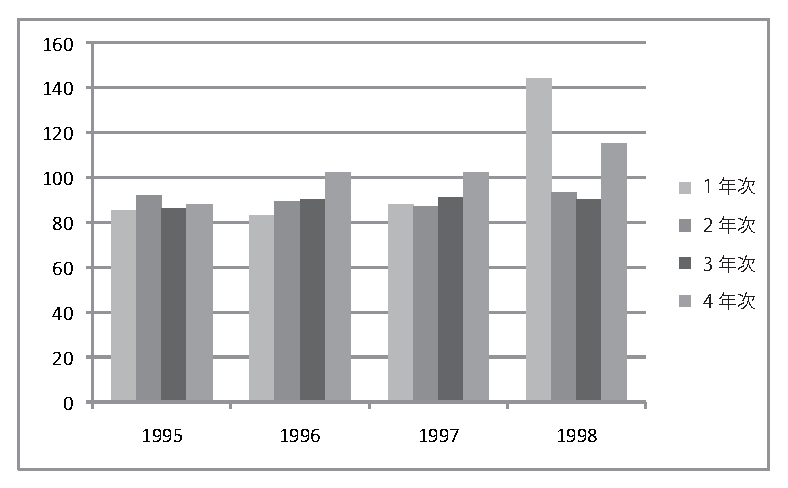
\includegraphics[width=3cm]{sample.eps}
\usepackage{epsfig} % for 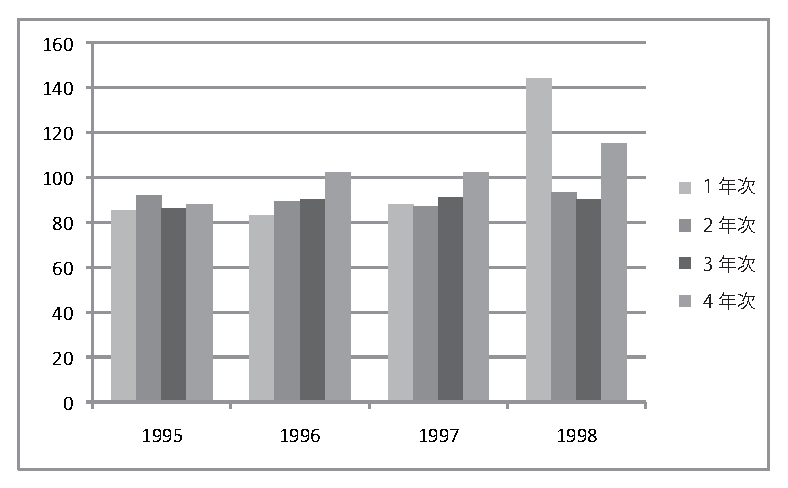
\psfig{file=sample.eps,width=3cm}
%\usepackage{epsf} % for \epsfile{file=sample.eps,scale=0.6}
%\usepackage{epsbox} % for \epsfile{file=sample.eps,scale=0.6}
\usepackage{/Users/takagihayata/workspace/materialize-mongodb/paper/mast/class/mediabb} % for pdf

\usepackage{times} % use Times Font instead of Computer Modern
% \usepackage{listings} % for soursecode
% \usepackage{plistings} % for soursecode
\usepackage{/Users/takagihayata/workspace/materialize-mongodb/paper/mast/class/docmute} % texファイル分割用

\setcounter{tocdepth}{3}
\setcounter{page}{-1}

\setlength{\oddsidemargin}{0.1in}
\setlength{\evensidemargin}{0.1in}
\setlength{\topmargin}{0in}
\setlength{\textwidth}{6in}
%\setlength{\textheight}{10.1in}
\setlength{\parskip}{0em}
\setlength{\topsep}{0em}

%\newcommand{\zu}[1]{{\gt \bf 図\ref{#1}}}

%% タイトル生成用パッケージ(重要)
\usepackage{/Users/takagihayata/workspace/materialize-mongodb/paper/mast/class/mast-jp-sjis}

%% タイトル
%% 【注意】タイトルの最後に\\ を入れるとエラーになります
\title{NoSQL型データベースシステムでの実体化ビュー選択に関する研究}
%% 著者
\author{髙木 颯汰}
%% 指導教員
\advisor{古瀬 一隆 陳 漢雄}

%% 年月 (提出年月)
%% 年月は必要に応じて書き替えてください.
\majorfield{ } \yearandmonth{2019年 1月}


\addtocounter{page}{2} %単体でコンパイルした際の調整用
\addtocounter{chapter}{1} %単体でコンパイルした際の調整用
\begin{document}

\chapter{関連技術}
\label{chap:LiteratureReview}
\section{Materialized View}
リレーショナルデータベースにおけるビュー (view) はリレーショナルデータモデルの発案者であるコッドにより導入された概念であり\cite{Codd1974RecentII},1つ以上の表(または他のビュー)から任意のデータを選択し,それらを表したものである.ビューの実体はデータを持たないSQL文であり,実行された際にはバックグラウンドでSELECT処理が毎回実行される.それに対して実体化ビュー(Materialized View)はビューと同じく複数の表の結合処理や集計処理を行うが,その結果を実際のテーブルに保持する.保持された実体化ビューは元のテーブルが更新されるたびに更新される.そのため,最新でない状態を取得する可能性はあるが,結合処理が必要ないため効率的なアクセスが可能になる.その一方,更新処理が増加するので実体化ビュー化する部分の選択は慎重に行う必要があり,この作業を自動化する研究が行われている\cite{mistry2001materialized}.図\ref{figure:MvDescription}は1対1のデータモデルの実体化ビューを図示したものである.
\begin{figure}[htbp]
	\begin{center}
		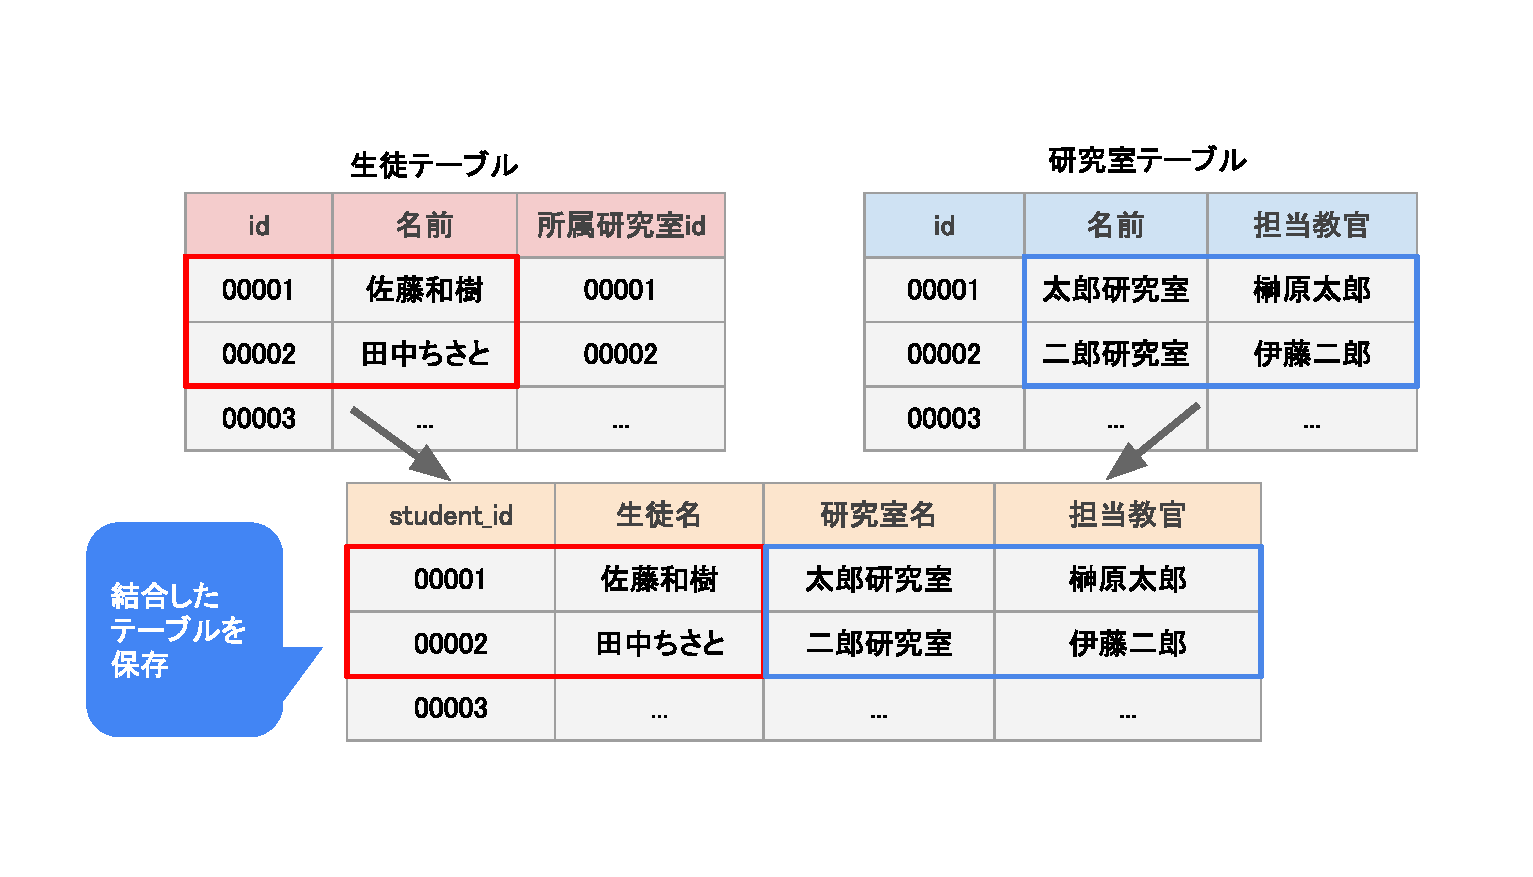
\includegraphics[width=32em, trim=0 5em 0 0]{src/MvDescription.eps} %[trim=left bottom right top]
	\end{center}
	\caption{実体化ビュー}
	\label{figure:MvDescription}
\end{figure}


多対多の結合を表す際には中間テーブルを用意してそれぞれのテーブルからレコードを結合する.その際の流れを図\ref{figure:MvDescription2}に示す.履修中間テーブルに生徒idと授業idを格納している.idが00001の生徒が履修している授業を取得する際には履修中間テーブルのstudent\_idが00001のレコードを取得し,付随するclass\_idを用いて授業の情報を取得する.結合元のテーブルのレコード数が無数にある場合には結合元テーブルでの検索時間が増加し,結合元のテーブルのレコード数の増加と共に中間テーブルのレコード数も増える傾向にあるので,中間テーブルでの検索時間も増加する.
\begin{figure}[htbp]
	\begin{center}
		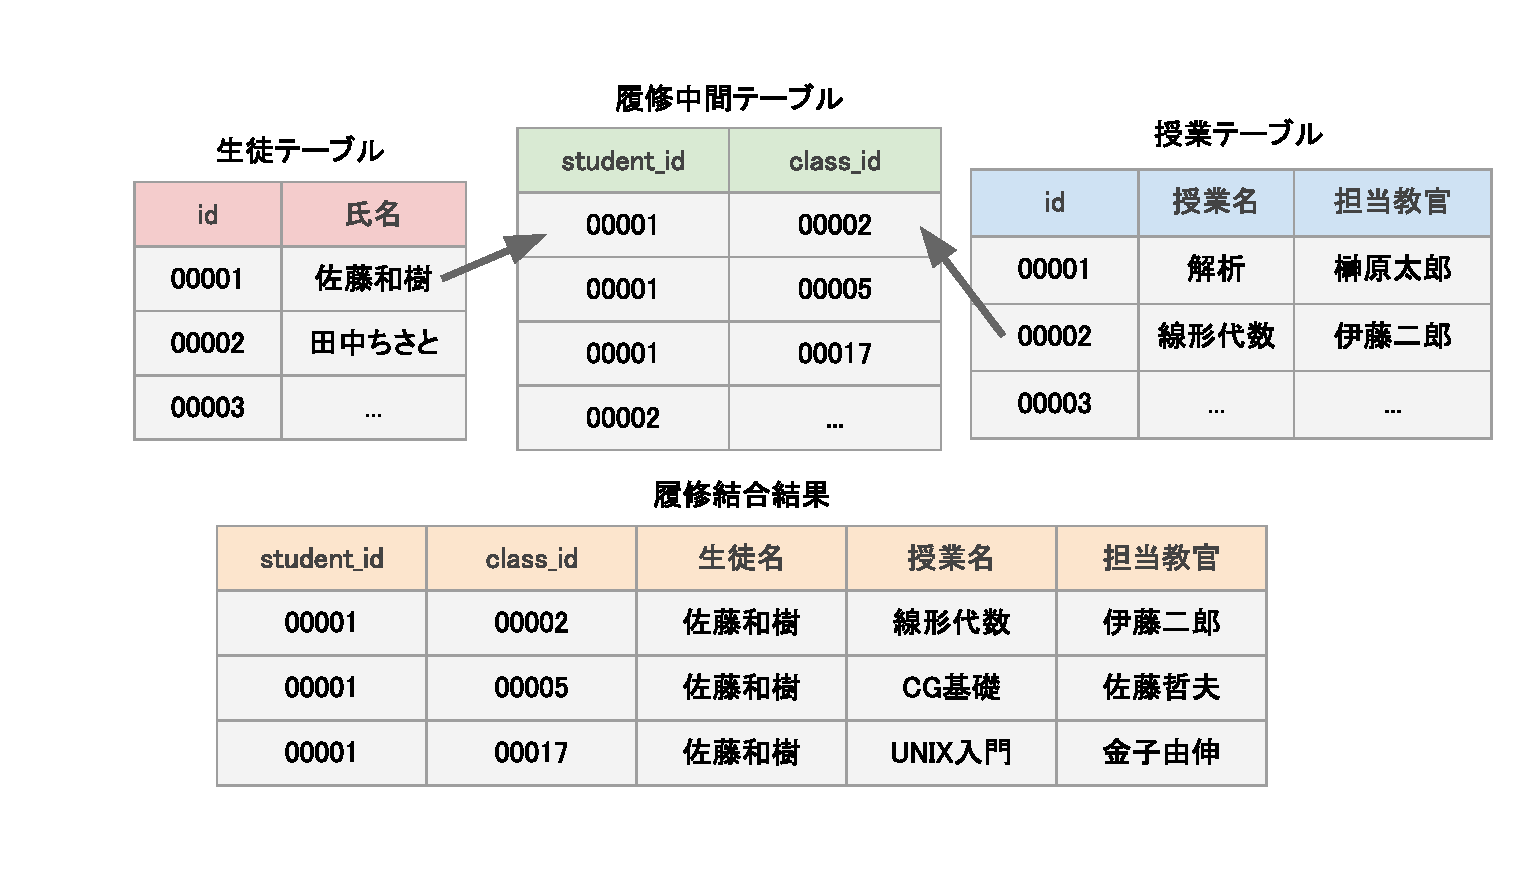
\includegraphics[width=32em, trim=0 5em 0 0]{src/MvDescription2.eps} %[trim=left bottom right top]
	\end{center}
	\caption{多対多の結合}
	\label{figure:MvDescription2}
\end{figure}

Materialized Viewを用いた際のメリットとして,結合処理や集計処理が不要になり高速化することに加え,問い合わせに用いるSQL文が簡素化することが挙げられる.表\ref{table:mv_sql}は図\ref{figure:MvDescription2}の生徒テーブルをstudent,授業テーブルをclass,履修中間テーブルをcourse\_selection,生徒の履修結合結果を得るために作成したMaterialized Viewをmv\_course\_selectionとした際に,idが00001の生徒が履修している授業を取得するSQL文をMaterialized Viewを使用する場合としない場合を比較したものである.
\begin{table}[htb]
  \begin{center}
    \caption{生徒テーブルと授業テーブルを結合するSQL}
		\label{table:mv_sql}
    \begin{tabular}{|l|l|} \hline
			\begin{tabular}{c}
				Materialized View\\不使用
			\end{tabular} &
			\begin{tabular}{l}
				SELECT student.id AS student\_id,
				class.id AS class\_id,\\
				student.name AS student\_name,
				class.name AS class\_name,\\
				class.teacher AS teacher\\
				FROM student, class, course\_selection \\
				WHERE course\_selection.student\_id = 00001 AND\\ course\_selection.student\_id = student.id AND\\ course\_selection.class\_id = class.id;\\
			\end{tabular}\\
			 \hline
			 \begin{tabular}{c}
 				Materialized View\\使用
 			\end{tabular} &
			\begin{tabular}{l}
				SELECT student\_id, class\_id, student\_name, class\_name, teacher\\
				FROM mv\_course\_selection\\
				WHERE student\_id = 00001;
			\end{tabular}
			\\ \hline
    \end{tabular}
  \end{center}
\end{table}

\section{NoSQL}
NoSQLとは,“Not only SQL”の略称であり,SQLを用いないデータベースの総称を表す \cite{太田201204}.情報の大規模化が進み,ビッグデータと呼ばれる概念が登場すると共に,構造が複雑な様々なデータが登場するようになった.NoSQLは,そのような複雑な構造のデータに柔軟に対応し処理を行うことができる.GoogleやAmazon,Twitterなど,世界的規模を誇る企業がNoSQLデータベースを利用しており,今後ますますデータの大規模化が進む現代社会において,重要な役割を果たすデータベースである\cite{太田201204}.
NoSQLデータベースはキー・バリュー型,カラム指向型,ドキュメント指向型,グラフ型の4種類の型に大別することができる.キー・バリュー型は,インデックスであるキーと値であるバリューのペアでデータが構成され,キーを指定することでデータを呼び出すことができる.カラム指向型は行に対してキーが付され,それが複数の列(カラム)に対応する形のデータモデルである.ドキュメント指向型は,JSONやXMLなどの形式で記述されたドキュメントの形でデータを扱うデータモデルである.グラフ型は,データ間の関係性をグラフの構造で表すデータモデルである\cite{太田201204}.

\section{MongoDB}
MongoDBとは,JSONやXMLなどの形式で記述されたドキュメント指向型のデータを扱うNoSQLデータベースの代表的なものの一つである.RDBとは違い,スキーマの定義を必要としない\cite{太田201204}\cite{mongodb}.また,JSON形式のデータを扱うため,Webシステムなどに利用しやすい.
MongoDBにおいては,RDBのテーブルにあたるものとしてコレクション,RDBの行にあたるものとしてドキュメント,RDBの列にあたるものとしてフィールドというデータ構想が使われる.

MongoDBではデータの格納にJSONをバイナリエンコーディングしたBSON形式を用いる\cite{Harrison201512}.RDBMSとMongoDBにおける一般的な検索のクエリを表\ref{table:RDB_Mongo_Find}に,更新のクエリを表\ref{table:RDB_Mongo_Update}に示す.
また,MongoDBはクエリの結果をJSON形式で返す.返却されるクエリセットの例を図\ref{MongoJson}に示す.
\begin{table}[htb]
  \begin{center}
    \caption{RDBMSとMongoDBにおける検索クエリ}
		\label{table:RDB_Mongo_Find}
    \begin{tabular}{|c|l|} \hline
			RDBMS &
			\begin{tabular}{l}
				SELECT *\\
				FROM comments\\
				WHERE story = "Next Generations";\\
			\end{tabular}\\ \hline
			MongoDB &
			\begin{tabular}{l}
				db.comments.find(\{\\
				\ \ story: "Next Generations"\\
				\});\\
			\end{tabular}\\ \hline
    \end{tabular}
  \end{center}
\end{table}
\begin{table}[htb]
  \begin{center}
    \caption{RDBMSとMongoDBにおける更新クエリ}
		\label{table:RDB_Mongo_Update}
    \begin{tabular}{|c|l|} \hline
			RDBMS &
			\begin{tabular}{l}
				UPDATE comments\\
				SET story = "Next Generations 2"\\
				WHERE story = "Next Generations";
			\end{tabular}\\ \hline
			MongoDB &
			\begin{tabular}{l}
				db.comments.update(\{\\
				\ \ story: "Next Generations"\\
				\}, \{\\
				\ \ \$set: \{story: "Next Generations 2"\}\\
				\});\\
			\end{tabular}\\ \hline
    \end{tabular}
  \end{center}
\end{table}

\begin{figure}[htbp]
	\begin{center}
		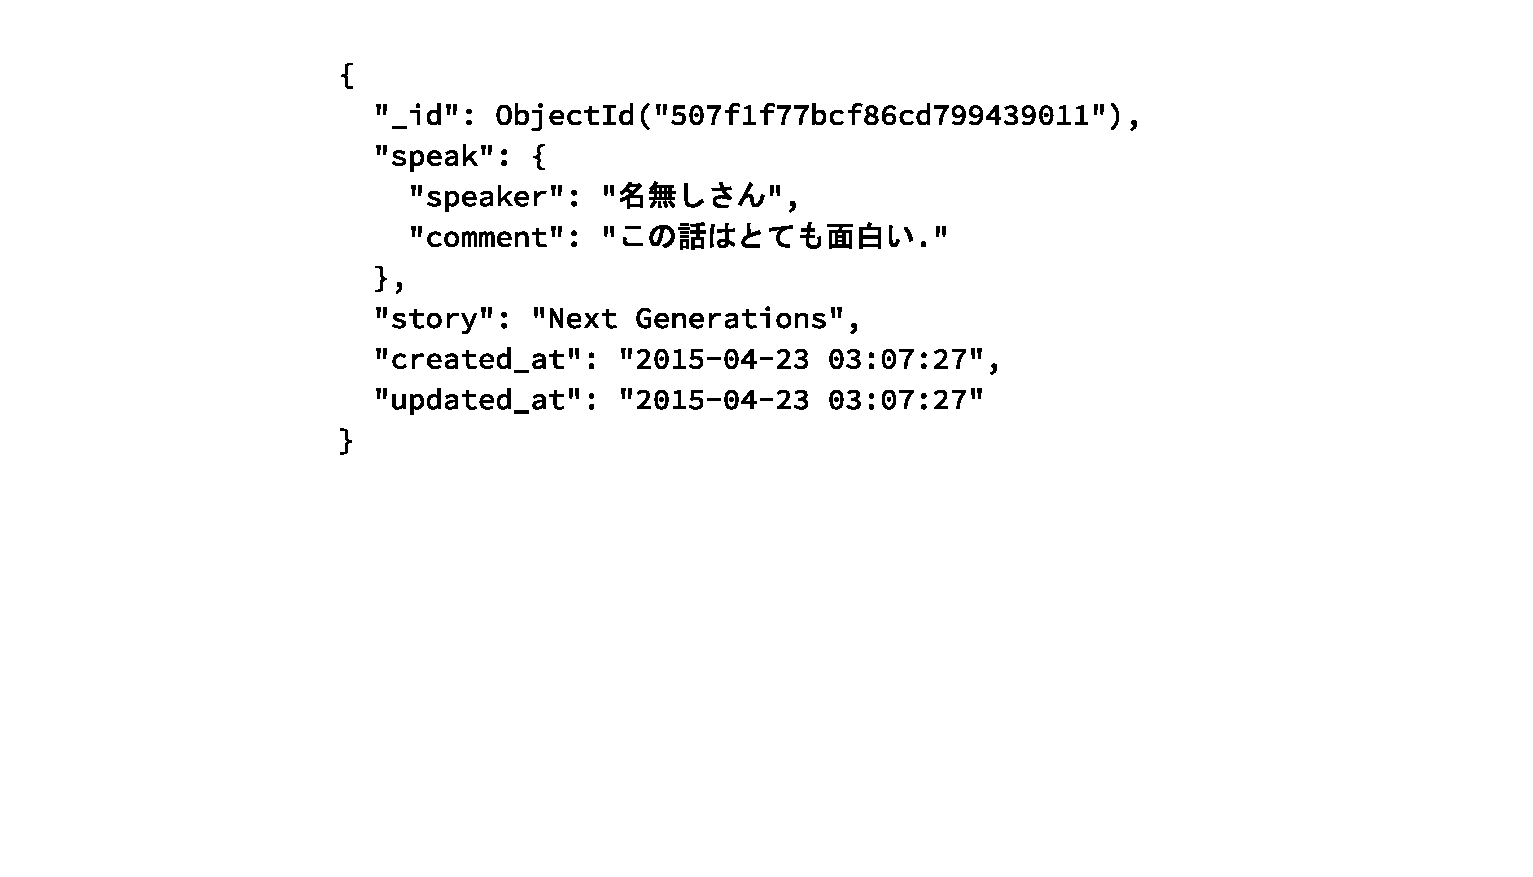
\includegraphics[width=30em, trim=10em 18em 10em 0em]{src/MongoJson.eps} %[trim=left bottom right top]
	\end{center}
	\caption{MongoDBから返されるクエリセットの例}
	\label{MongoJson}
\end{figure}



\section{Restful API}
RESTとはRoy Fieldingが提唱した概念であり\cite{fielding2000architectural},“REpresentational State Transfer”の略である.分散システムにおける複数のソフトウェアを連携させるのに適した考え方であり,やりとりされる情報はそれ自体で完結して解釈できるステートレス性,全てのリソースが一意的なアドレスを持つアドレス可能性,他の基盤的な機能を用いずに別の情報や状態を含むことで他のリソースを参照できる持続性,HTTPメソッド(“GET”や“POST”など)の統一インターフェースを提供していることなどの原則から成る.RESTの原則に則り構築されたHTTPの呼び出しインターフェースをRESTful APIと呼ぶ.本論文ではRESTful APIをミドルウェアに実装し実験を行う.


\end{document}
